\subsection{2026-09-22 --- Structural diagnosis of the count model: width, head, stationarity}
\label{sec:diagnosis}

\subsubsection*{What we did}

Six consecutive attempts to improve the count model returned noise or harm: the v2 water-balance
fixes ($-0.0030$, Section~\ref{sec:v2rejected}), properly-encoded categorical unit identity
($-0.0042$), per-unit historical marginals ($-0.0020$), feature pruning at four thresholds
($\pm 0.002$), raw-feature forwarding ($-0.0110$, Section~\ref{sec:orthogonal}) and stacking
($+0.0001$, Section~\ref{sec:stacked}). That pattern is not six unlucky ideas. Before adding a
seventh feature block we stopped and measured the architecture itself, asking three questions
that had never been checked:

\begin{enumerate}
  \item How much of the count model's input actually varies with the unit being scored?
  \item Is ``mixed'' a single regression target, or several?
  \item How much of the model's importance sits on features that will not look the same in the
        2023--24 test period?
\end{enumerate}

The diagnostic is \texttt{/tmp/diag\_wide.py}; the fixes it motivated are
\texttt{src/count\_model.py}.

\subsubsection*{Finding 1 --- the count model is largely blind to which unit it is scoring}

\begin{finding}
Of 437 input features, only \textbf{60 vary with the unit}. The remaining \textbf{377 are
identical across all 14 units of a case}, and they carry \textbf{72.6\% of the model's
importance}. All within-case discrimination --- which is most of what micro-average ROC-AUC
rewards --- must come from the 60 unit-specific columns, on 27.4\% of the attention.
\end{finding}

\begin{figure}[h]\centering
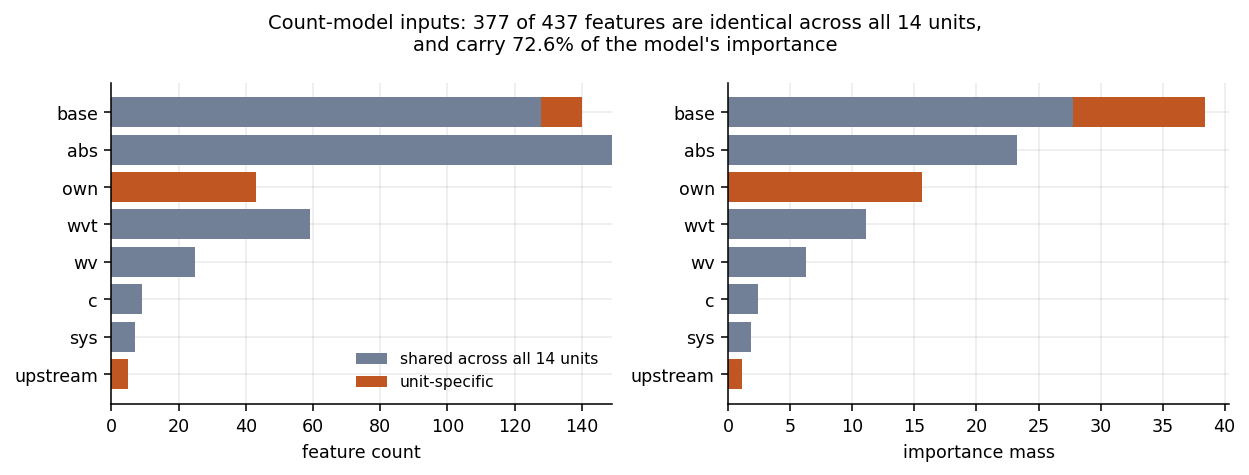
\includegraphics[width=\textwidth]{figures/diag_01_shared_vs_unitspecific.png}
\caption{Count-model input composition by feature group, by count and by importance mass.
Grey is shared across all 14 units of a case; orange is unit-specific. See
\texttt{figures.md}, id \texttt{diag\_01\_shared\_vs\_unitspecific}.}
\end{figure}

The mechanism is an assembly error rather than a modelling one.
\texttt{unit\_relative.build\_unit\_relative} already resolves each plant's columns into
\texttt{own\_}/\texttt{upstream\_}/\texttt{sys\_} form --- that was the whole point of
Section~\ref{sec:unitrel}. But the experiment scripts then merged every plant's columns straight
back in under \texttt{abs\_}, \texttt{c\_} and \texttt{wvt\_} prefixes, re-introducing exactly
the sharing the resolution had removed. The \texttt{abs\_} block alone is 149 columns, all
shared, carrying 23.2\% of importance.

A shared feature can only move a whole case up or down. It cannot say that Lio should run this
week and Songa should not. This is a clean structural explanation for why the same four units
(Lio, Songa, Haukeli, Hogga) stay broken regardless of what we add: they are bad \emph{relative
to other units in the same week}, and that is the one thing the input is weakest at expressing.

\supersededby{sec:abcd}{the measurement holds, but this inference does not: removing the shared
block costs $-0.0285$, and absolute features help monotonically the more of them are kept}

\paragraph{This also reinterprets an earlier result.} We concluded that explicit unit identity
``does not help'' because adding a categorical \texttt{unit\_cat} cost $-0.0042$. The better
reading is that identity is \emph{already} being paid for: with 377 shared columns, the tree
must burn splits rediscovering which unit a row belongs to before any shared feature can be used
differentially. Adding an identity column does not relieve that cost, it adds to it.

\subsubsection*{Finding 2 --- ``mixed'' is bimodal, so the single regressor predicts a hole}

The head is a 3-class model (all-off / mixed / all-on) plus one regressor fitted to the count
within mixed weeks. That assumes the mixed count is unimodal. It is not.

\begin{figure}[h]\centering
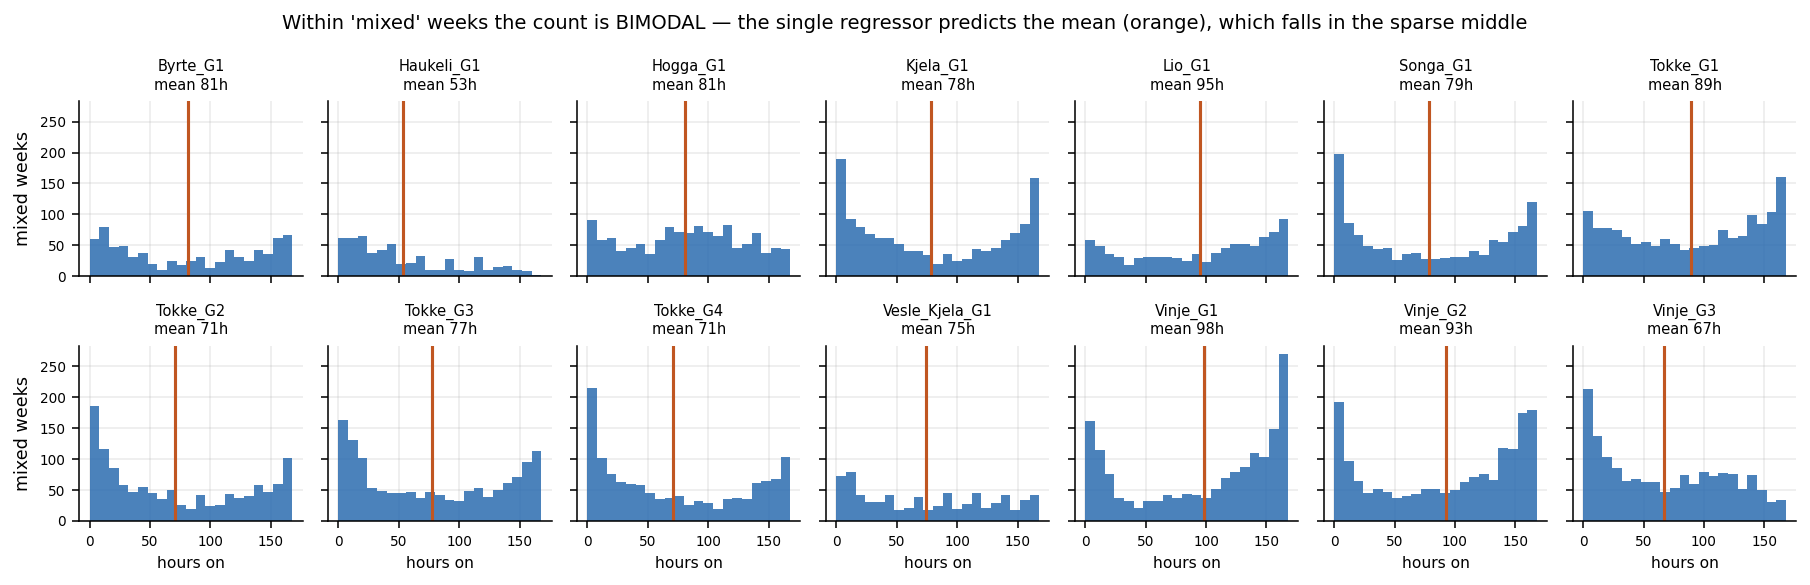
\includegraphics[width=\textwidth]{figures/diag_02_mixed_bimodality.png}
\caption{Distribution of hours-on within \emph{mixed} weeks, per unit, with the fitted mean in
orange. Most units are U-shaped. See \texttt{figures.md}, id \texttt{diag\_02\_mixed\_bimodality}.}
\end{figure}

\begin{center}\small
\begin{tabular}{lrrrrrr}
\toprule
unit & p25 & p50 & p75 & $<$56h & $>$112h & \textbf{middle third} \\
\midrule
Kjela\_G1  & 19 & 67  & 140 & 0.457 & 0.374 & \textbf{0.170} \\
Tokke\_G4  & 14 & 56  & 134 & 0.500 & 0.324 & \textbf{0.176} \\
Vinje\_G1  & 36 & 118 & 152 & 0.291 & 0.529 & \textbf{0.180} \\
Songa\_G1  & 17 & 74  & 140 & 0.432 & 0.381 & \textbf{0.187} \\
Hogga\_G1  & 43 & 83  & 117 & 0.305 & 0.294 & 0.401 \\
\bottomrule
\end{tabular}
\end{center}

\begin{finding}
For most units only \textbf{17--24\% of ``mixed'' weeks fall in the middle third} of the range.
``Mixed'' is really \emph{barely-on} plus \emph{barely-off} with a thin gap between. A single
regressor fitted to a bimodal target returns the conditional mean, which lands in the sparse
middle --- precisely where the truth almost never is. Kjela's mixed weeks cluster near 20h and
near 145h; predicting 78h is wrong by roughly 55h in both directions.
\end{finding}

This is the first mechanism we have found for the 24h count MAE that is not ``we need more
features''. It is a specification error in the head, and it is fixable by classifying over count
bins and carrying the whole predicted distribution forward instead of collapsing it to a point
estimate.

\subsubsection*{Finding 3 --- the drift is real but narrow, and confined to absolute levels}

Screening every feature for distribution shift between 2015--18 and 2019--22:

\begin{center}\small
\begin{tabular}{lrr}
\toprule
feature & drift (SD) & $|$corr with time$|$ \\
\midrule
\texttt{price\_back\_1y}     & 0.80 & 0.57 \\
\texttt{price\_vol\_back\_1y}& 0.79 & 0.57 \\
\texttt{price\_f1m}          & 0.76 & 0.59 \\
\texttt{price\_std}          & 0.72 & 0.53 \\
\texttt{wv\_f1w}             & 0.69 & 0.52 \\
\midrule
\texttt{own\_mean\_spread}   & \textbf{0.35} & 0.24 \\
\texttt{spread\_frac\_pos}   & \textbf{0.19} & 0.10 \\
\bottomrule
\end{tabular}
\end{center}

\begin{finding}
No importance mass sits on features drifting more than 1.0 SD, and only \textbf{14.1\%} on
features drifting more than 0.5 SD. But \emph{every} high-drift feature is an absolute price or
water-value level (the 2021--22 energy crisis), and \emph{every} stationary one is a difference
or ratio of two co-drifting quantities. Spread $=$ price $-$ water value, and the drift cancels.
\end{finding}

\begin{figure}[h]\centering
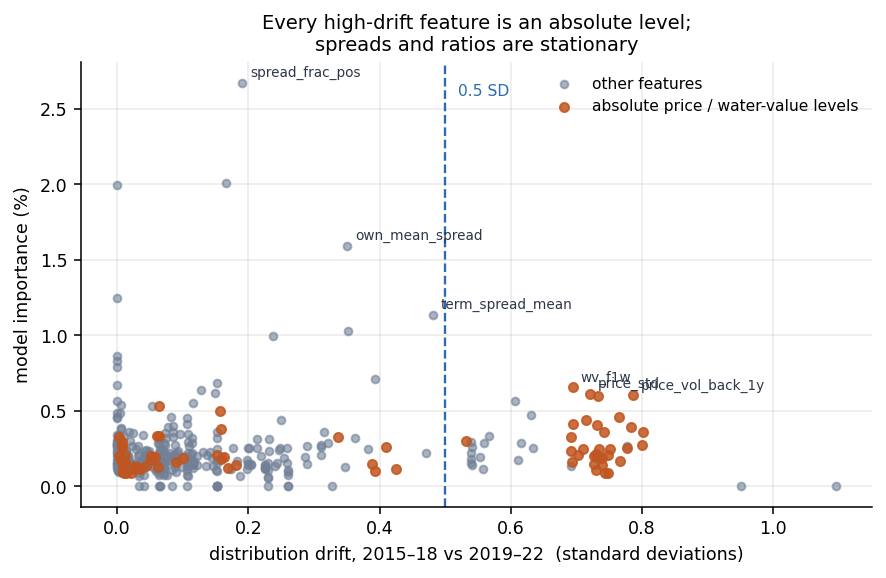
\includegraphics[width=0.72\textwidth]{figures/diag_03_stationarity_drift.png}
\caption{Importance against distribution drift. See \texttt{figures.md}, id
\texttt{diag\_03\_stationarity\_drift}.}
\end{figure}

We already benefited from this by accident: the pruned top-15 of Section~\ref{sec:pruning} were
\emph{all} spreads, margins and break-evens, with no raw price column surviving. We found the
principle empirically without naming it. Naming it gives a construction rule --- split a level
feature into a stationary shape (ratio to a trailing reference) plus an explicitly quarantined
level --- which matters because the test period sits on the far side of the crisis.

\subsubsection*{A constraint that rules out a whole family of fixes}

Checking coverage of every source settled a question that had been open since the marginals
experiment:

\begin{center}\small
\begin{tabular}{lll}
\toprule
source & coverage & \\
\midrule
\texttt{Unit\_commitment\_decisions} & 2015-01-01 -- 2022-12-31 & \textbf{targets} \\
test cases                            & 2023-01-01 -- 2024-12-25 & 725 cases, zero overlap \\
\texttt{Historical\_inflow}           & 1958 -- 2025 & 594k rows \\
\texttt{Historical\_volume}, \texttt{Synthetic\_water\_value} & 2015 -- 2025-01-01 & \\
\texttt{Constraint\_min\_flow/volume} & 2015 -- 2025 & \\
\bottomrule
\end{tabular}
\end{center}

\begin{finding}
The test set is \textbf{strictly future}: 2023--24, with no case start shared with training.
Targets stop at 2022-12-31. Any feature derived from historical on/off labels is therefore
\textbf{12--24 months stale at prediction time and near-constant across all 725 test cases}.
This is the mechanism that made per-unit historical marginals backfire worst on Haukeli
($-0.024$), whose base rate collapsed from 0.87 to 0.14 within the training window.
\end{finding}

This retires the reweighting / oversampling / historical-prior family as normally constructed.
The surviving version is \emph{conditional}: $E[\text{count} \mid \text{state deciles}]$ is a
response surface rather than a base rate, and transfers under the weaker assumption that the
physical relationship is stable even when the marginal is not.

It also means the walk-forward protocol of Section~\ref{sec:wf2} is the structurally correct
one and a leave-one-out variant would be optimistic --- it would let the model interpolate
across a held-out block using data from both sides, which the submission can never do. We had
provisionally planned to switch to leave-one-out; that plan is dropped for this reason.

\subsubsection*{Unused data}

Two sources are present and under-used. \texttt{Historical\_inflow} covers \textbf{1958--2025},
but every seasonal-percentile feature computes its reference distribution from the case dates
(2015 onward) --- roughly eight years of a 67-year record. And the two constraint files are
joined as raw series but never resolved into \emph{which unit is obliged to pass the water},
which is the form in which a minimum-flow obligation would explain always-on behaviour for a
specific unit.

\subsubsection*{What this implies}

Four changes, implemented in \texttt{src/count\_model.py} and tested in
Section~\ref{sec:abcd}:

\begin{description}
  \item[A. Width.] Resolve the per-plant blocks into own/upstream/\emph{downstream} (the last
    was missing entirely), and convert the remaining cross-plant information into the unit's
    \emph{rank}, \emph{z-score} and \emph{share} among plants --- unit-specific and scale-free
    where the absolute columns were shared and drifting. Section~\ref{sec:unitrel} found
    relative$+$absolute beat relative alone, so we test \emph{reduced} absolute rather than
    none.
  \item[B. Head.] Classify over six count bins and forward the whole distribution.
  \item[C. Stationarity.] Split drifting levels into shape $+$ quarantined level.
  \item[D. Groups.] Structural (never label-derived) group attributes, since unit count
    distributions sort by merit order within a plant.
\end{description}
